\documentclass{book}

%Quitar páginas en blanco
\let\cleardoublepage\clearpage
\usepackage{etoolbox}
\makeatletter
\patchcmd{\@endpart}{\vfil\newpage}{\par}{}{}
\makeatother

\usepackage[spanish]{babel}
% Redefinir el título del índice
\addto\captionsspanish{
	\renewcommand{\contentsname}{Índice}
}

\usepackage[bookmarks,bookmarksopen,bookmarksdepth=3]{hyperref}
\usepackage{graphicx}
\usepackage{float}
\usepackage{subcaption}
\usepackage[left=4cm, right=4cm]{geometry}
\usepackage{enumitem}
\usepackage{palatino}
\usepackage{parskip}
\usepackage{amsthm}
\usepackage{amssymb}
\usepackage[nointegrals]{wasysym}%I was getting some problem "\iint already defined"
\usepackage{amsmath}
\usepackage{tikz}
\usepackage{tikz-cd}
\usetikzlibrary{%
	matrix,%
	calc,%
	arrows%
}

%\usepackage[style=nature]{biblatex}
\usepackage[nottoc,numbib]{tocbibind}%This is to include the References in the ToC. For some reason it is not working so I add it manually at the end of the document.
%\addbibresource{bib.bib}
\hypersetup{
	colorlinks=false,
	hidelinks
}

\theoremstyle{definition}
\newenvironment{Proof}[1][Proof]
{\proof[#1]\leftskip=1cm\rightskip=1cm}{\endproof}

\newtheorem*{defn}{Definición}
\newtheorem{defs}{Definiciones}
\newtheorem*{lema}{Lema}
\newtheorem*{obs}{Observación}
\newtheorem*{teo}{Teorema}
\newtheorem*{prop}{Proposición}
\newtheorem{coro}{Corolario}
\newtheorem*{coro*}{Corolario}
\newtheorem*{ejer}{Ejercicio}
\newtheorem*{pregunta}{Pregunta}

\newcommand{\R}{\mathbb{R}}
\newcommand{\Z}{\mathbb{Z}}
\newcommand{\N}{\mathbb{N}}
\newcommand{\C}{\mathbb{C}}
\newcommand{\Q}{\mathbb{Q}}
\newcommand{\T}{\mathbb{T}}
\newcommand{\K}{\mathbb{K}}
\DeclareMathOperator{\coker}{coker}
\DeclareMathOperator{\img}{img}

\renewcommand{\chaptername}{Parte}

\title{Notas de Topología Algebraica}
\author{Prof. Luis Jorge Sánchez Saldaña\\ \\ Notas por Dani}

\begin{document}
	\maketitle
	\tableofcontents
	
	\part{Grupo fundamental}
	
	\part{Espacios cubrientes}
	
	\part{Homología}
	\chapter{Álgebra Homológica}
	\section{Conceptos básicos}
	En este capítulo $R$ denotará un anillo asociativo con unidad (no necesariamente conmutativo). Normalmente pensaremos que es alguno de los siguientes: $\Z, \Q, \R$.
	
	Recordemos que un $R$-módulo es básicamente un espacio vectorial pero los escalares están $R$.
	\begin{defn}
		Un \textbf{$R$-complejo de cadenas} es una sucesión de $R$-módulos y homomorfismos
		\[\begin{tikzcd}
			(C_\bullet,\partial):= \quad \cdots \arrow{r} & C_p \arrow{r}{\partial_p} & C_{p-1} \arrow{r}{\partial_{p-1}} & C_{p-2} \arrow{r} & \cdots
		\end{tikzcd}\]
		tal que $\partial_{p-1}\partial_p=0$ para toda $p\in \mathbb{Z}$, que es equivalente a que $\text{img }\partial_p\subseteq\ker{\partial_{p-1}}$.
	\end{defn}
	
	\begin{defn}
		Un \textbf{morfismo de $R$-complejos de cadenas} es $(C_\bullet{},\partial)\to(D_\bullet{},\delta)$ es una sucesión de $R$-homomorfismos $C_p\xrightarrow[]{f_p} D_p$ tal que el siguiente diagrama conmuta:
		\[
		\begin{tikzcd}
			\cdots \arrow{r} & C_{p+1} \arrow{r}{\partial_{p+1}} \arrow{d}{f_{p+1}} & C_p \arrow{r}{\partial_p} \arrow{d}{f_p} & C_{p-1} \arrow{r} \arrow{d}{f_{p-1}} & \cdots \\
			\cdots \arrow{r} & D_{p+1} \arrow{r}{\delta_p} & D_p \arrow{r}{\delta_p} & D_{p-1} \arrow{r} & \cdots
		\end{tikzcd}
		\]
		es decir $f_{p-1}\partial_p=\delta_pf_p$ para toda $p\in\mathbb{Z}$.
	\end{defn}
	\begin{defn}
		Decimos que $(D_\bullet,\delta)$ es un \textbf{subcomplejo de cadenas} de $(C_\bullet,\partial)$ si $D_p\leq C_p$ para toda $p\in\mathbb Z$ y $\partial|_{D_p}=\delta_p$. El cociente $(C_\bullet/D_\bullet,\partial)$ es el complejo de cadenas dado por
		\[
		\begin{tikzcd}
			\cdots \arrow{r} & C_{p+1}/D_{p+1} \arrow{r}{\partial_{p+1}} & C_{p}/D_{p} \arrow{r}{\partial_{p}} & C_{p-1}/D_{p-1} \arrow{r} & \cdots
		\end{tikzcd}
		\]
		donde los mapeos frontera son de la forma $\partial_p/\delta_p([c])=[\partial_p(c)]$.
	\end{defn}
	\begin{defn}\leavevmode
		\begin{itemize}
			\item Los elementos en $C_p$ se llaman \textbf{cadenas de dimensión $p$}.
			\item Los elementos en $\ker\partial_p:=Z_p$ se llaman \textbf{ciclos de dimensión $p$}.
			\item Los elementos en $\text{img }\partial_{p+1}:=F_p:=B_p$ se llaman \textbf{fronteras de dimensión $p$}.
		\end{itemize}
	\end{defn}
	
	\begin{defn}
		El \textbf{$p$-ésimo grupo de homogía} de $(C_{\bullet{}},d)$ es
		$$H_p(C_{\dot{}}):=Z_p/B_p=\ker\partial_p/\text{img }\partial_{p+1}$$
		Y decimos que dos ciclos $c$ y $c'$ son \textbf{homólogos} si $[c]=[c']\in H_p(C_\bullet)$.
	\end{defn}
	Veamos una figura de dos ciclos homólogos:
	\begin{figure}[H]
		\centering
		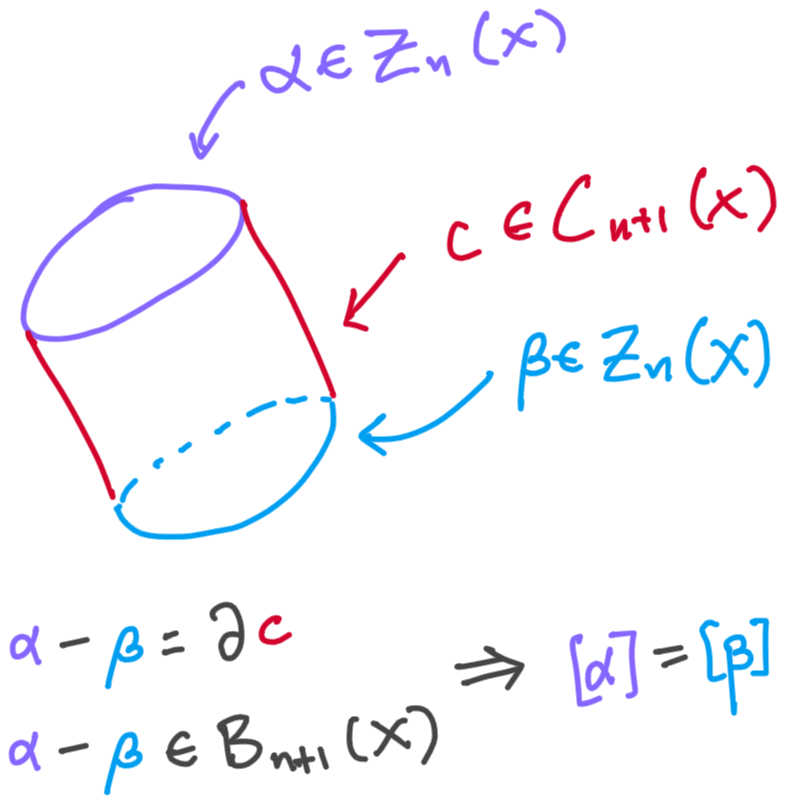
\includegraphics[width=0.4\linewidth]{Homología/H1.png}
	\end{figure}
	\begin{ejer}[Función inducida]
		Si $(C_\bullet{},\partial)\xrightarrow f(C'_\bullet{},\partial')$ es un homeomorfismo, entonces $f(Z_p)\subseteq Z'_p$ y $f(B_p)\subseteq B'_p$ así que la función inducida
		\begin{align*}
			\bar f_p:H_p(C_\bullet{})\to & H_p(C_\bullet{})\\
			a+B_p\mapsto& f_p(a)+B'_p
		\end{align*}
		está bien definida.
		Si además tenemos un segundo homomorfismo $(C'_\bullet,\partial')\xrightarrow{g}(C''_\bullet,\partial'')$, entonces $\overline{g\circ f}=\bar g\circ\bar f$. Y por último, $\overline{Id}_{C_p}=Id_{H_p(C)}$.
	\end{ejer}
	Con este ejercicio comenzamos a ver las propiedades funtoriales de la homología, aunque por ahora no profundizaremos en este lenguaje.
	\section{Sucesiones exactas}
	\begin{defn}
		Decimos que la sucesión 
		\[
		\begin{tikzcd}
			\cdots \arrow{r} & C_p \arrow{r}{f_p} & C_{p-1} \arrow{r}{f_{p-1}} & C_{p-2} \arrow{r} & \cdots
		\end{tikzcd}
		\]
		es \textbf{exacta en $C_p$} si  $\text{img }f_p=\ker{f_{p-1}}$. Y la sucesión es \textbf{exacta} si es exacta en todos los $C_p$. Esto sucede si y sólo si $H_p(C_\bullet{})=0$ para todo $p\in\mathbb{Z}$.
	\end{defn}
	\begin{obs}\leavevmode
		\begin{itemize}
			\item El grupo de homología mide qué tan lejos está la sucesión de ser exacta.
			\item La sucesión puede ser "finita", o sea pueden haber muchos módulos que son cero.
		\end{itemize}
	\end{obs}
	\begin{defn}
		Una sucesión exacta de la forma $$0\to P\to Q\to R\to 0$$ se llama \textbf{sucesión exacta corta}. Las sucesiones exactas infinitas en ambas direcciones se llaman \textbf{sucesiones exactas largas}.
	\end{defn}
	\begin{prop}\leavevmode
		\begin{enumerate}
			\item $0\to A\xrightarrow{\alpha}B$ es exacta si y sólo si $\ker{\alpha}=0$, es decir $\alpha $ es inyectiva.
			\item $A\xrightarrow{\alpha}B\to 0$ es exacta si y sólo si $\text{img }{\alpha}=B$, es decir $\alpha $ es suprayectiva.
			\item $0\to A\xrightarrow{\alpha}B\to 0$ es exacta si y sólo si $\alpha $ es un isomorfismo por los dos incisos anteriores.
			\item $0\to A\xrightarrow{\alpha}B\xrightarrow{\beta} C\to0$ es exacta si y sólo si $\alpha$ es inyectiva, $\beta$ es suprayectiva y $\ker\beta=\text{img }\alpha$, de manera que $\beta$ induce un isomorfismo $C\cong B/\text{img }\alpha$.\par
			Si pensamos que $\alpha$ es la inclusión de $A$ como subgrupo de $B$, podemos escribir $C\cong B/A$ .
		\end{enumerate}
	\end{prop}
	\begin{obs}[Primer teorema de isomorfismo] Si $M'\subseteq M$, entonces
		\[
		\begin{tikzcd}
			0 \arrow{r} & M' \arrow[hookrightarrow]{r} & M \arrow[twoheadrightarrow]{r} & M/M' \arrow{r} & 0
		\end{tikzcd}
		\]
		es una sucesión exacta.
	\end{obs}
	\section{Homotopía}
	\begin{defn}
		Dos homomorfismos 
		\begin{align*}
			f,g:(C_\bullet,\partial)\to(C'_\bullet,\partial')
		\end{align*}
		son \textbf{homotópicos} si existen homomorfismos $H_p:C_p\to C'_{p+1}$ para toda $p\in\Z$ tales que $$f_p-g_p=\partial'_{p+1}H_p+H_{p-1}\partial_p$$ Estas flechas se pueden visualizar aquí:
		\[
		\begin{tikzcd}
			\cdots \arrow{r} & C_{p+1} \arrow{r}{\partial_{p+1}} \arrow{d}[left]{f_{p+1}-g_{p+1}} & C_p \arrow{r}[blue]{\partial_p} \arrow{d}[right,red]{f_p-g_p} \arrow{ld}[left,blue]{H_p} & C_{p-1} \arrow{r} \arrow{d}[right]{f_{p-1}-g_{p-1}} \arrow{ld}[right,blue]{H_{p-1}} & \cdots \\
			\cdots \arrow{r} & C'_{p+1} \arrow{r}[below,blue]{\partial'_{p+1}} & C'_p \arrow{r}[below]{\partial_p'} & C'_{p-1} \arrow{r} & \cdots
		\end{tikzcd}
		\]
		Así que la suma de las flechas azules es igual a la flecha roja. (No estamos diciendo que el diagrama sea conmutativo).
	\end{defn}
	\begin{lema}
		Con la notación de arriba, $\bar f_p=\bar g_p:H_p(C_\bullet)\to H_(C'_\bullet)$. Es decir, funciones homotópicas inducen funciones iguales en homología.
	\end{lema}
	\section{El lema de la serpiente}
	\begin{lema}[de la serpiente]Consideremos el diagrama conmutativo de $R$-módulos y supongamos que sus filas son exactas:
		\[
		\begin{tikzcd}
			&Z_1'\arrow{r}{\phi'}\arrow{d}{\partial_1}&Z_2'\arrow{r}{\psi'}\arrow{d}{\partial_2}&Z_3'\arrow{r}\arrow{d}{\partial_3}&0\\
			0\arrow{r}&Z_1\arrow{r}[below]{\phi}&Z_2\arrow{r}[below]{\psi}&Z_3&
		\end{tikzcd}
		\]
		Entonces existe un homomorfismo $\delta_*:\ker\partial_3\to Z_1/\img\partial_1$ tal que
		\[\begin{tikzcd}
			\ker\partial_1\arrow{r}{\phi''}&\ker\partial_2\arrow{r}{\phi''}&\ker\partial_3\arrow{r}{\delta_*}&Z_1/\img\partial_1\arrow{r}{\bar\phi}&Z_2/\img\partial_2\arrow{r}{\bar\psi}&Z_3/\img\partial_3
		\end{tikzcd}\]
		es exacta, donde $\phi''$ y $\psi''$ son las restricciones de $\phi'$ y $\psi'$, y $\bar\phi$ y $\bar\psi$ son homomorfismos inducidos por $\phi$ y $\psi$. ¿Dónde está la serpiente?
	
		
		\[\begin{tikzpicture}
			\matrix[matrix of math nodes,column sep={60pt,between origins},row
			sep={60pt,between origins},nodes={asymmetrical rectangle}] (s)
			{
				&|[name=ka]| \ker \partial_1 &|[name=kb]| \ker \partial_2 &|[name=kc]| \ker \partial_3 \\
				%
				&|[name=A]| Z_1' &|[name=B]| Z_2' &|[name=C]| Z_3' &|[name=01]| 0 \\
				%
				|[name=02]| 0 &|[name=A']| Z_1 &|[name=B']| Z_2 &|[name=C']| Z_3 \\
				%
				&|[name=ca]| \coker \partial_1 &|[name=cb]| \coker \partial_2 &|[name=cc]| \coker \partial_3 \\
			};
			\draw     (ka) edge (A)
			(kb) edge (B)
			(kc) edge (C)
			(A) edge node[auto] {\(\phi'\)} (B)
			(B) edge node[auto] {\(\psi'\)} (C)
			(C) edge (01)
			(A) edge node[auto] {\(\partial_1\)} (A')
			(B) edge node[auto] {\(\partial_2\)} (B')
			(C) edge node[auto] {\(\partial_3\)} (C')
			(02) edge (A')
			(A') edge node[auto] {\(\phi\)} (B')
			(B') edge node[auto] {\(\psi\)} (C')
			(A') edge (ca)
			(B') edge (cb)
			(C') edge (cc)
			;
			\draw[gray,dashed] (ka) edge node[auto] {\(\phi''\)}(kb)
			(kb) edge node[auto] {\(\psi''\)}(kc)
			(ca) edge node[auto] {\(\bar\phi\)} (cb)
			(cb) edge node[auto] {\(\bar\psi\)} (cc)
			;
			\draw[gray,dashed,rounded corners] (kc) -| node[auto,text=black,pos=.7]
			{\(\partial_*\)} ($(01.east)+(.5,0)$) |- ($(B)!.35!(B')$) -|
			($(02.west)+(-.5,0)$) |- (ca);
		\end{tikzpicture}\]
		donde $\coker\partial_i=Z_i/\partial_i$. (En la versión \href{https://tex.stackexchange.com/questions/3892/how-do-you-draw-the-snake-arrow-for-the-connecting-homomorphism-in-the-snake-l}{\textbf{original}} de este diagrama sí están las flechas).
	\end{lema}
	\begin{obs}
		Intuitivamente, el $\coker$ nos da información de qué tan lejos está un homomorfismo de ser suprayectivo.
	\end{obs}
\chapter{El teorema fundamental del álgebra homológica}
\section{Teorema fundamental del álgebra homológica}
	Primero introduciremos algo de notación
	\begin{defn}
		Diremos que una sucesión de complejos de cadena
		\[\begin{tikzcd}
			&\cdots\arrow{r}&C_\bullet\arrow{r}{f}&D_\bullet\arrow{r}{g}&E_\bullet\arrow{r}&\cdots
		\end{tikzcd}\]
		es exacta en $D_\bullet$ si 
		\[\begin{tikzcd}
			&\cdots\arrow{r}&C_p\arrow{r}{f_p}&D_p\arrow{r}{g_p}&E_p\arrow{r}&\cdots
		\end{tikzcd}\]
		es exacta para todo $p\in\Z$
	\end{defn}
	\begin{teo}[fundamental del álgebra homológica]
		Si 
		\[\begin{tikzcd}
			&\cdots\arrow{r}&A_\bullet\arrow{r}{\phi}&B_\bullet\arrow{r}{\psi}&C_\bullet\arrow{r}&\cdots
		\end{tikzcd}\]
		es una sucesión exacta de complejos de cadena, entonces existen homomorfismos $$\partial_{*p}:H_p(C.)\to H_{p-1}(A.)$$
		tales que la sucesión
		\[\begin{tikzcd}
			&\cdots\arrow{r}&H_p(A_\bullet)\arrow{r}{\bar\phi_p}&H_p(B_\bullet)\arrow{r}{\bar\psi_p}&H_p(C_\bullet)\arrow{r}{\delta_{*p}}&H_{p-1}(A_\bullet)\arrow{r}{\bar\phi_{p-1}}&H_{p-1}(B_\bullet)\arrow{r}&\cdots
		\end{tikzcd}\]
		es exacta.
	\end{teo}
	En el siguiente diagrama conmutativo se ve claramente qué está pasando:
	\[
	\begin{tikzcd}
		& & 0 \arrow{d} & 0 \arrow{d} & 0 \arrow{d} & \\
		& \cdots \arrow{r} & A_{p+1} \arrow{r}{\partial_{p+1}} \arrow{d}{i_{p+1}} & A_p \arrow{r}{\partial_p} \arrow{d}{i_p} & A_{p-1} \arrow{r} \arrow{d}{i_{p-1}} & \cdots \\
		& \cdots \arrow{r} & B_{p+1} \arrow{r}{\partial_{p+1}} \arrow{d}{j_{p+1}} & B_p \arrow{r}{\partial_p} \arrow{d}{j_p} & B_{p-1} \arrow{r} \arrow{d}{j_{p-1}} & \cdots \\
		& \cdots \arrow{r} & C_{p+1} \arrow{r}{\partial_{p+1}} \arrow{d} & C_p \arrow{r}{\partial_p} \arrow{d} & C_{p-1} \arrow{r} \arrow{d} & \cdots \\
		& & 0 & 0 & 0 & \\
	\end{tikzcd}
	\]

\section{Natrualidad del homomorfismo de conexión}
\begin{teo}[Naturalidad del homomorfismo de conexión]
	\[\begin{tikzcd}
		&0\arrow{r}&A_\bullet\arrow{r}{i}\arrow{d}{f}&B_\bullet\arrow{r}{j}\arrow{d}{g}&C_\bullet\arrow{r}\arrow{d}{h}&0\\
		&0\arrow{r}&A'_\bullet\arrow{r}&B'_\bullet\arrow{r}&C'_\bullet\arrow{r}&0
	\end{tikzcd}\]
	donde las filas son exactas.\par
	Entonces, el siguiente diagrama conmuta
		\[\begin{tikzcd}
		&\cdots\arrow{r}&H_p(A)\arrow{r}\arrow{d}{\bar f}&H_p(B)\arrow{r}\arrow{d}{\bar g}&H_p(C)\arrow{r}{\delta_*}\arrow{d}{\bar h}&H_{p-1}(A)\arrow{r}\arrow{d}{\bar f}&H_{p-1}(B)\arrow{r}\arrow{d}{\bar g}&H_{p-1}(C)\arrow{r}\arrow{d}{\bar h}&\cdots\\
		&\cdots\arrow{r}&H_p(A')\arrow{r}&H_p(B')\arrow{r}&H_p(C')\arrow{r}&H_{p-1}(A')\arrow{r}&H_{p-1}(B')\arrow{r}&H_{p-1}(C')\arrow{r}&\cdots
		\end{tikzcd}\]
		(Para acomodar este diagrama \href{https://tex.stackexchange.com/questions/663056/wide-tikz-cd-diagram-not-centered-shifted-to-the-right}{\textbf{aquí hay soluciones}})
\end{teo}

	
\end{document}
